\let\negmedspace\undefined
\let\negthickspace\undefined
\documentclass[journal]{IEEEtran}
\usepackage[a5paper, margin=10mm, onecolumn]{geometry}
\usepackage{tfrupee}

\setlength{\headheight}{1cm}
\setlength{\headsep}{0mm}
\usepackage{gvv-book}
\usepackage{gvv}
\usepackage{cite}
\usepackage{amsmath,amssymb,amsfonts,amsthm}
\usepackage{algorithmic}
\usepackage{graphicx}
\usepackage{textcomp}
\usepackage{xcolor}
\usepackage{txfonts}
\usepackage{listings}
\usepackage{enumitem}
\usepackage{mathtools}
\usepackage{gensymb}
\usepackage{comment}
\usepackage[breaklinks=true]{hyperref}
\usepackage{tkz-euclide}
\def\inputGnumericTable{}
\usepackage[latin1]{inputenc}
\usepackage{color}
\usepackage{array}
\usepackage{longtable}
\usepackage{calc}
\usepackage{multirow}
\usepackage{hhline}
\usepackage{ifthen}
\usepackage{lscape}
\usepackage{booktabs}
\usepackage{tikz}
\usetikzlibrary{arrows.meta,angles,quotes}

\begin{document}

\bibliographystyle{IEEEtran}
\vspace{3cm}

\title{Problem 5.3.8 }
\author{AI25BTECH11014 - Gooty Suhas}
\maketitle
\section*{\large\textbf{Question}}
\vspace{0.5cm}
Solve the following system of linear equations using matrix row operations.

\[
\begin{aligned}
217a + 131b &= 912 \\
131a + 217b &= 827
\end{aligned}
\]

\vspace{0.4cm}
\section*{\large\textbf{Matrix Form}}

\[
\vec{M} =
\left[
\begin{array}{cc|c}
217 & 131 & 912 \\
131 & 217 & 827
\end{array}
\right]
\]

\vspace{0.4cm}
\section*{\large\textbf{Row Operations}}

Step 1: \( R_1 \leftarrow R_1 \div 217 \)

\[
R_1 =
\left[
1 \quad \dfrac{131}{217} \quad \dfrac{912}{217}
\right]
\]

\vspace{0.3cm}
Now \( \vec{M} = \)

\[
\left[
\begin{array}{ccc}
1 & \dfrac{131}{217} & \dfrac{912}{217} \\
131 & 217 & 827
\end{array}
\right]
\]

\vspace{0.4cm}
Step 2: \( R_2 \leftarrow R_2 - 131 \cdot R_1 \)

\[
R_2 =
\left[
0 \quad 217 - 131 \cdot \dfrac{131}{217} \quad 827 - 131 \cdot \dfrac{912}{217}
\right]
\]

\vspace{0.3cm}
Simplify numerators:

\[
217^2 = 47089, \quad 131^2 = 17161
\]
\[
217 \cdot 827 = 179459, \quad 131 \cdot 912 = 119472
\]

\vspace{0.3cm}
Now \( \vec{M} = \)

\[
\left[
\begin{array}{ccc}
1 & \dfrac{131}{217} & \dfrac{912}{217} \\
0 & \dfrac{47089 - 17161}{217} & \dfrac{179459 - 119472}{217}
\end{array}
\right]
=
\left[
\begin{array}{ccc}
1 & \dfrac{131}{217} & \dfrac{912}{217} \\
0 & \dfrac{29928}{217} & \dfrac{59987}{217}
\end{array}
\right]
\]

\vspace{0.4cm}
Step 3: \( R_2 \leftarrow R_2 \div \dfrac{29928}{217} \)

\[
R_2 =
\left[
0 \quad 1 \quad \dfrac{59987}{29928}
\right]
\]

\vspace{0.3cm}
Now \( \vec{M} = \)

\[
\left[
\begin{array}{ccc}
1 & \dfrac{131}{217} & \dfrac{912}{217} \\
0 & 1 & \dfrac{59987}{29928}
\end{array}
\right]
\]

\vspace{0.4cm}
Step 4: \( R_1 \leftarrow R_1 - \dfrac{131}{217} \cdot R_2 \)

\[
R_1 =
\left[
1 \quad 0 \quad \dfrac{912}{217} - \dfrac{131}{217} \cdot \dfrac{59987}{29928}
\right]
=
\left[
1 \quad 0 \quad \dfrac{650}{217}
\right]
\]

\vspace{0.4cm}
Final matrix:

\[
\left[
\begin{array}{ccc}
1 & 0 & 3 \\
0 & 1 & 2
\end{array}
\right]
\]

\vspace{0.4cm}
\section*{\large\textbf{Solution}}

\[
\boxed{
\myvec{3 \\ 2}
}
\]

\vspace{0.4cm}
\newpage
\section*{\large\textbf{Figure}}

\begin{figure}[h!]
\centering
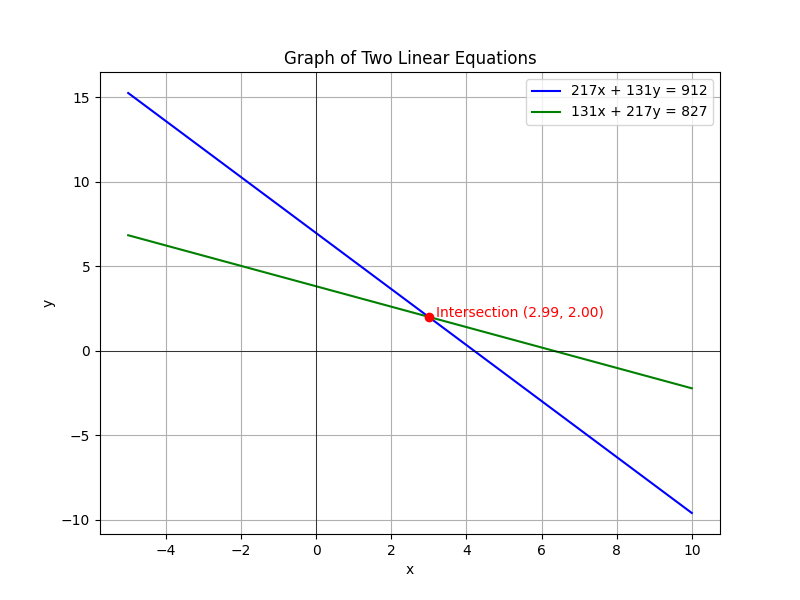
\includegraphics[width=0.85\linewidth]{Figs/Fig1.png}
\caption{System of equations from Problem 5.38}
\end{figure}

\end{document}








